\chapter{Выполнение работы}

Для достижения поставленной цели необходимо:
\begin{enumerate}
	\item изменить код common\_struct.h под индивидуальное задание;
	\item изменить код хост--подсистемы под индивидуальное задание;
	\item реализовать алгоритм поиска ближайшего значения к заданному в sw\_kernel;
	\item реализовать общий алгоритм нахождения суммы значений из заданного промежутка в sw\_kernel.
\end{enumerate}

\section{Изменение кода common\_struct.h}

В листинге \ref{lst:common} представлен измененный код common\_struct.h.
\begin{lstlisting}[caption={Измененный код common\_struct.h}, label={lst:common}, language={c++}]
#ifndef COMMON_STRUCT
#define COMMON_STRUCT

#ifdef __riscv64__
#include "map.h"
#endif
#include "compose_keys.hxx"

//Номера структур данных в SPE
enum Structures : uint32_t {
	null            = 0,   	//Нулевая структура не используется
	users_pnum    	= 1,	//Таблица 1 
	resources_pnum  = 2,	//Таблица 2 
	function_pnum = 3 // Рабочая таблица 3
};

#ifdef __riscv64__
//Задание даипазонов и курсоров
template<typename Range>
struct reverse {
	Range r;
	[[gnu::always_inline]] reverse(Range r) : r(r) {}
	[[gnu::always_inline]] auto begin() {return r.rbegin();}
	[[gnu::always_inline]] auto end() {return r.rend();}
};

template<typename K, typename V>
struct Handle {
	bool ret_val;
	K k{get_result_key<K>()};
	V v{get_result_value<V>()};
	[[gnu::always_inline]] Handle(bool ret_val) : ret_val(ret_val) {
	}
	
	[[gnu::always_inline]] operator bool() const {
		return ret_val;
	}
	
	[[gnu::always_inline]] K key() const {
		return k;
	}
	
	[[gnu::always_inline]] V value() const {
		return v;
	}
};
#endif


//////////////////////////////////////
// Описание формата ключа и значения
//////////////////////////////////////


struct users {
	using vertex_t = uint32_t;
	int struct_number;
	constexpr users(int struct_number) : struct_number(struct_number) {}
	static const uint32_t idx_bits = 32;
	static const uint32_t idx_max = (1ull << idx_bits) - 1;
	static const uint32_t idx_min = idx_max; 
	
	//Запись для формирования ключей (* - наиболее значимые биты поля)
	STRUCT(key)
	{
		uint32_t	idx	    :idx_bits;	//Поле 0:
		uint32_t	user    :32; 		//Поле 1*
	};
	
	//Запись для формирования значений
	STRUCT(val)
	{
		uint32_t	role	:32;		//Поле 0:
		time_t		time    :32; 		//Поле 1*
	};
	//Обязательная типизация
	#ifdef __riscv64__
	DEFINE_DEFAULT_KEYVAL(key, val)
	#endif
};

struct rev_function{
	using vertex_t = uint32_t;
	int struct_number;
	constexpr rev_function(int struct_number) : struct_number(struct_number) {}
	static const uint32_t idx_bits = 32;
	static const uint32_t idx_max = (1ull << idx_bits) - 1;
	static const uint32_t idx_min = idx_max; 
	
	//Запись для формирования ключей (* - наиболее значимые биты поля)
	STRUCT(key)
	{
		uint64_t	idx	    :64;	//Поле 0:
	};
	
	//Запись для формирования значений
	STRUCT(val)
	{
		uint64_t	value	:64;		//Поле 0:
	};
	//Обязательная типизация
	#ifdef __riscv64__
	DEFINE_DEFAULT_KEYVAL(key, val)
	#endif
};

constexpr users USERS(Structures::users_pnum);
constexpr rev_function REV_FUNCTION(Structures::function_pnum);

#endif //COMMON_STRUCT
\end{lstlisting}

\section{Изменение кода хост--подсистемы}

В листинге \ref{lst:host} представлен измененный код хост--подсистемы.
\begin{lstlisting}[caption={Измененный код хост--подсистемы}, label={lst:host}, language={c++}]
#include <iostream>
#include <random>
#include <iterator>
#include <string>
#include <regex>
#include <sstream>
#include <fstream>
#include <ctime>
#include "host_main.h"

#define KEYS_COUNT 13
#define MIN_VALUE 356
#define MAX_VALUE 10000

using namespace std;

int main(int argc, char** argv)
{
	ofstream log("task.log"); //поток вывода сообщений
	unsigned long long offs=0ull;
	gpc *gpc64_inst; //указатель на класс gpc
	
	std::random_device dev;
	std::mt19937 rng(dev());
	std::uniform_int_distribution<std::mt19937::result_type> gen_int(MIN_VALUE, MAX_VALUE);
	
	//Инициализация gpc
	if (argc<2) {
		log<<"Использование: host_main <путь к файлу rawbinary>"<<endl;
		return -1;
	}
	
	//Захват ядра gpc и запись sw_kernel
	gpc64_inst = new gpc();
	cout<<"Открывается доступ к "<<gpc64_inst->gpc_dev_path<<endl;
	if (gpc64_inst->load_swk(argv[1])==0) {
		cout<<"Программное ядро загружено из файла "<<argv[1]<<endl;
	}
	else {
		cout<<"Ошибка загрузки sw_kernel файла << argv[1]"<<endl;
		return -1;
	}
	
	//Инициализация таблицы для вложенного запроса
	gpc64_inst->start(__event__(update)); //обработчик вставки 
	
	for (uint64_t i = 0, key=MIN_VALUE;i<KEYS_COUNT;++i, ++key) {
		uint64_t val = key * key;
		gpc64_inst->mq_send(rev_function::key{.idx=key}); //запись о роли #idx
		gpc64_inst->mq_send(rev_function::val{.value=val}); //роль и время доступа
		std::cout << "inserting by key " << key << " value " << val << std::endl;
	}
	
	//Терминальный символ
	gpc64_inst->mq_send(-1ull);
	std::cout << "finished sending\n";
	gpc64_inst->start(__event__(select)); //обработчик запроса поиска 
	std::cout << "started selecting\n";
	bool requested = true;
	while (requested)
	{
		std::cout << "Введите x1 для поиска суммы значений на промежутке (x1, x2):(-1 для завершения ввода)\n";
		uint64_t val_1;
		std:: cin >> val_1;
		
		if (val_1 == (uint64_t)-1)
		{
			requested = false;
			break;
		}
		
		std::cout << "Введите x2 для поиска суммы значений на промежутке (x1, x2):(-1 для завершения ввода)\n";
		uint64_t val_2;
		std:: cin >> val_2;
		
		if (val_2 == (uint64_t)-1)
		{
			requested = false;
			break;
		}
		
		gpc64_inst->mq_send(val_1);
		gpc64_inst->mq_send(val_2);
		
		uint64_t result = gpc64_inst->mq_receive();
		uint64_t result_val = rev_function::val::from_int(result).value;
		std:: cout<< "\n Сумма:" << result_val << "\n";
	}
	
	gpc64_inst->mq_send(-1ull);
	
	
	std::cout << "Выход!" << endl;
	return 0;
}
\end{lstlisting}

\section{Реализация алгоритма поиска ближайшего значения к заданному}

В листинге \ref{lst:alg1} представлена реализация алгоритма поиска ближайшего значения к заданному.
\begin{lstlisting}[caption={Листинг реализации алгоритма поиска ближайшего значения к заданному}, label={lst:alg1}, language={c++}]
void get_nearest_value(uint64_t &key, uint64_t &val, bool need_bigger) {
	if (need_bigger) {
		auto g = REV_FUNCTION.ngr(rev_function::key{.idx=key});
		key = g.key();
		val = g.value();
	} else {
		auto l = REV_FUNCTION.nsm(rev_function::key{.idx=key});
		key = l.key();
		val = l.value();
	}
}
\end{lstlisting}

\section{Реализация общего алгоритма нахождения суммы значений из заданного промежутка}

В листинге \ref{lst:alg2} представлена реализация общего алгоритма нахождения суммы значений из заданного промежутка.
\begin{lstlisting}[caption={Листинг реализации общего алгоритма нахождения суммы значений из заданного промежутка}, label={lst:alg2}, language={c++}]
void select() {
	while(1) {
		uint64_t val;
		uint64_t key_1 = mq_receive();
		if (key_1 == -1)
			break;
		
		uint64_t key_2 = mq_receive();
		if (key_2 == -1)
			break;
		
		get_nearest_value(key_2, val, false);
		get_nearest_value(key_1, val, true);
		
		if (key_1 && key_2) {
			uint64_t summ = val;
			
			for (uint64_t i = key_1; i < key_2;) {
				get_nearest_value(i, val, true);
				summ += val;
			}
			
			mq_send(summ);
		}
		else
			break;
	}
}
\end{lstlisting}

\chapter{Пример работы программы}

На рисунке \ref{img:demo} продемонстрирована работа программы.
\begin{figure}[ht!]
	\centering
	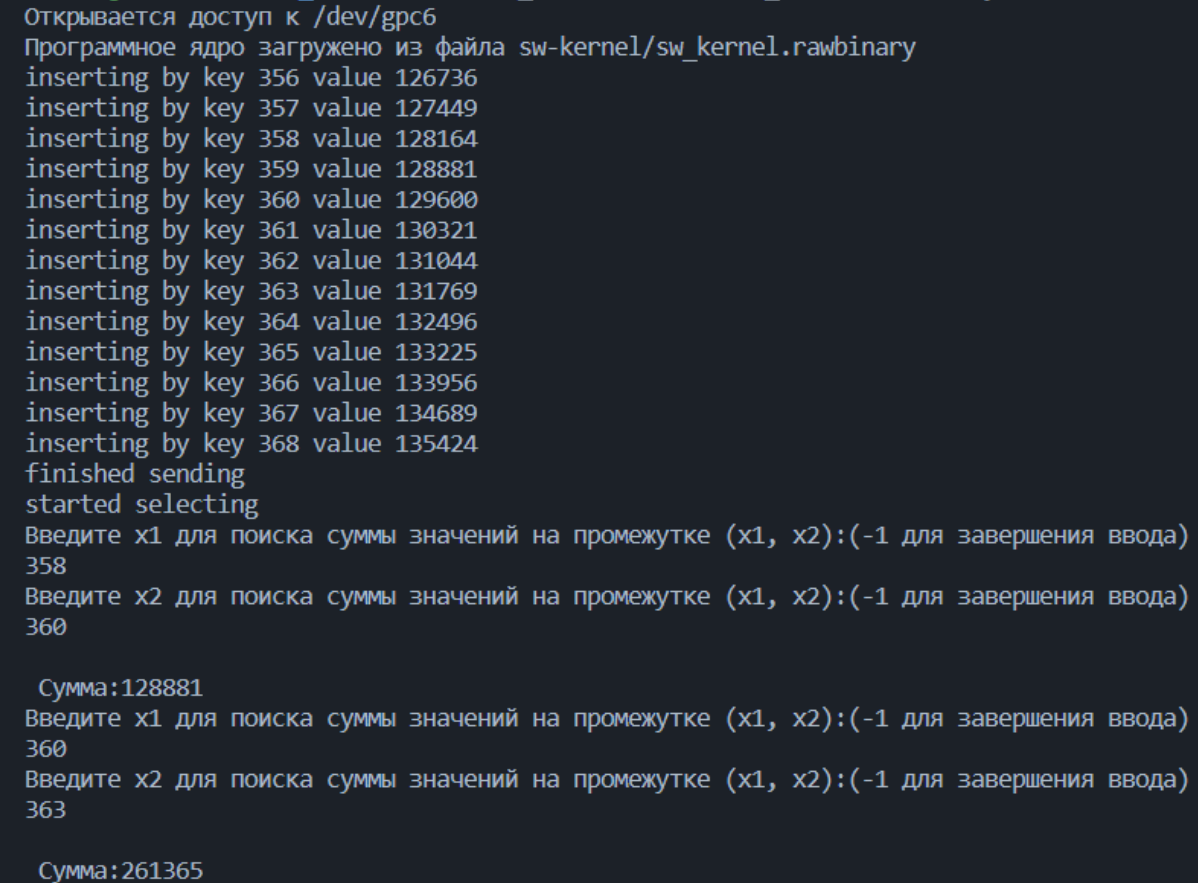
\includegraphics[width=170mm]{./img/demo.png}
	\caption{Демонстрация работы программы}
	\label{img:demo}
\end{figure}